%!TEX root = ./dp7-application.tex
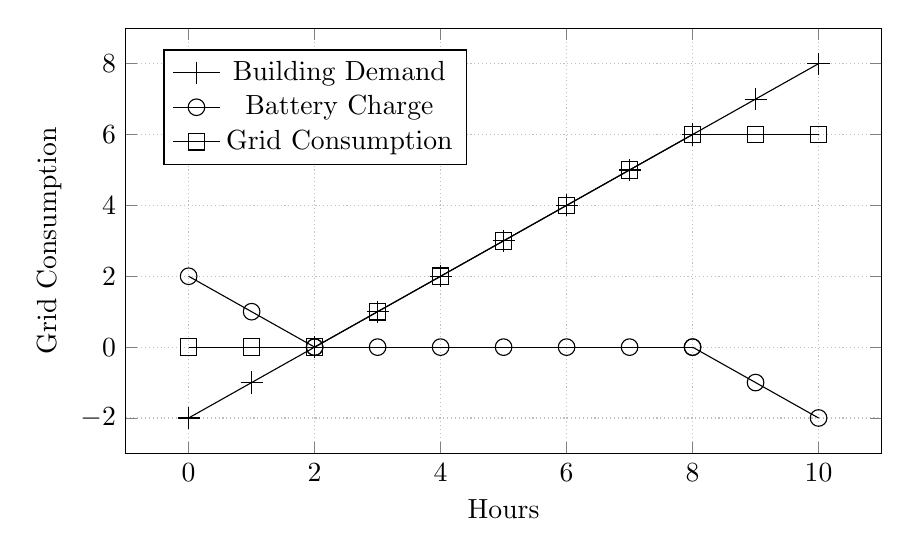
\begin{tikzpicture}

\begin{axis}[
x=0.8cm,y=0.45cm,
xlabel=Hours,
ylabel=Grid Consumption,
grid=both, grid style={style=densely dotted},
legend style={at={(0.05,0.95)},anchor=north west}
] 

% Draw the Demand-Supply curve
\addplot[mark=+,mark size=4] expression[domain=0:10,samples=11] {x-2};
\addlegendentry{Building Demand} 

% Draw the Battery curve
\addplot[mark=o,mark size=3] expression[forget plot,domain=0:2,samples=3] {2-x}; 
\addplot[mark=o,mark size=3] expression[forget plot,domain=2:8,samples=7] {0}; 
\addplot[mark=o,mark size=3] expression[domain=8:10,samples=3] {8-x}; 
\addlegendentry{Battery Charge} 

% Draw the Grid supply curve
\addplot[mark=square,mark size=3] expression[forget plot,domain=0:2,samples=3] {0}; 
\addplot[mark=square,mark size=3] expression[forget plot,domain=2:8,samples=7] {x-2}; 
\addplot[mark=square,mark size=3] expression[domain=8:10,samples=3] {6}; 
\addlegendentry{Grid Consumption} 
\end{axis} 
\end{tikzpicture} 
